% !TEX root = thesis.tex

\section{Methodology}\label{sec:style}

As we've seen in the previous section the log data comprises of error messages of multiple unknown classes. The basic idea is to analyse the data present and cluster the messages in to different classes. One can see from the error logs that a few features of all the messages are unique (eg. timestamps, ErrorID.. etc). These unique features are given lesser priority in the clustering of the data  hence corresponding weights are assigned to these features. The distance between the messages is compared by ignoring these unique features. The trivial logic is to put the messages whose distance is less than a predefined threshold are put into the same class. A dummy illustration of the algorithm is shown below. 

\begin{figure}[htp]
    \centering
    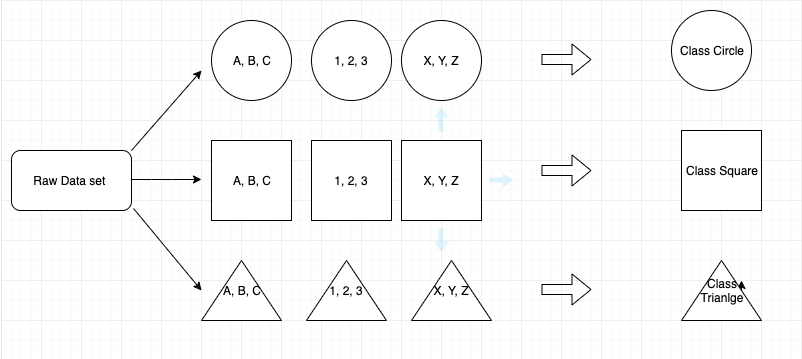
\includegraphics[width=7cm]{img/proc.png}
    \caption{Illustration of the log data analysis procedure}
    \label{fig:galaxy}
\end{figure}

The figure shows the demonstration of the clustering and the classification procedure. Each one of the 3 shapes represents as class and the variables inside each shape represent the unique features in the dataset. The data is clustered based on how similar the shapes are ignoring the unique features of the message. Once the messages are clustered, the principal features are extracted from each class and marked as a feature vector of that class. Now, every new entry in the data point is compared with these principal feature vectors to 

The first step idea is to extract message "keys" which
correspond to messages generated by the same lines of code but with different message variables, implemented using regex. They proceed to utilise
the similarity in clustering raw log keys by using the edit distance as their
metric, which is defined as the number of insertion, deletion or replacement
operations required to convert one message into another. This distance does
not account for the position of the words in the logs, and so they use the
weighted edit distance which uses sigmoid function to place greater emphasis on words appearing earlier in the message than later based on the
idea/observation that programmers tend to place important information in
this way. The edit distances to all other logs is calculated, and all members
whose distance is less than a threshold is connected via a link. 

In this section, we define how we approach the problem
mathematically, starting with our choice of similarity measure, the Jaccard
Similarity, J: in order to identify similar items, we must first identify how
to define and quantify similarity. We progress to describe shingling, a naïve
method to fully iterate over the parameter space in order to compute J, and
learn how it is infeasible to apply to large datasets, such as when hundreds
of thousands of logs are generated every minute, as can be the case in distributed systems.

\subsection{Min hash}\label{sec:_academic_style}
In order to identify similar items, a similarity measure is necessary. A common and intuitive means is that of the Jaccard Similarity. This treats two strings as sets of words, and defines the size of their intersection relative to their union as the defining metric of similarity. We therefore see that not only can the relation between two logs be evaluated,but the distances between different logs represent hierarchies of similarity, and these can be mined to reveal underlying clusters. Other alternative methods include measuring distance as the number of edits required to transform one message in another. he signatures we desire to construct for sets are composed of the results of a large number of calculations, say several hundred, each of which is a “minhash”. To minhash a set represented by a column of the characteristic matrix, pick
a permutation of the rows. The minhash value of any column is the number of
the first row, in the permuted order, in which the column has a 1. The probability that the minhash function for a random permutation of
rows produces the same value for two sets equals the Jaccard similarity
of those sets. \textbf{[Add reference for minhash here]}


\subsection{Min Hash Locality Sensitive Hashing}\label{sec:_tips_for_writing}

MinHash is an effective means for reducing the dimensionality of variable
length alphanumerical data to fixed length numerical output, with which
Jaccard similarity can be probabilistically calculated via random sampling.
However, each log hash must still be compared to every other in order to
identify relationships, resulting in complexity O(n**2). There are a range of
search methods for identifying nearest neighbours (examples, references)
based on space partitioning but it was shown that they all degrade to linear search for sufficiently high dimensions. Locality Sensitive Hashing
is used to reduce the search space by using hash collisions as a proxy for
similarity.  \textbf{{[Add reference for LSH here]}}

\subsection{Shingling}\label{sec:_tips_for_writing}
